\documentclass[titlepage]{article}
\usepackage{graphicx}
\usepackage{indentfirst}
\usepackage{array}
\usepackage{gensymb}
\usepackage{pdfpages}
\usepackage[bottom]{footmisc}
\usepackage[title,titletoc,toc]{appendix}
\renewcommand{\thetable}{\Roman{table}}
\renewcommand{\baselinestretch}{1.35}
\usepackage[margin=1in]{geometry}
\setlength{\parindent}{.4in}

\usepackage{fancyhdr} 
\pagestyle{fancy}
\lhead{\textsf{Design and Flight Analysis of the Remote-Controlled Flappy Bird Aircraft}}
\rhead{\textsf{\thepage}}
\cfoot{}
\renewcommand{\headrulewidth}{0.4pt}
\renewcommand{\footrulewidth}{0.4pt}

\begin{document}
\title{\textbf{Design and Flight Analysis of the Remote-Controlled Flappy Bird Aircraft}}
\author{Brian Quinn, Mark Paluta, Eliseo Miranda, Patrick Wall}
\date{May 9, 2014}
\maketitle

\begin{abstract}
Scale model, remotely-controlled aircraft are used extensively for hobby pilots, but also serve a secondary, educative purpose of allowing university students to apply aerodynamic theory to a physical flight application. In this design project, a high aspect ratio, low wing loading aircraft was designed to fly a mission in which it would be required to fly to high altitudes before performing an unpowered descent back to its cruising altitude. Implementing performance characteristics calculated using principles of fluid mechanics and aerodynamics, along with historical data from previous designs, the team of student engineers designed a minimalist vehicle, constructed from light woods and carbon fiber, that demonstrated speeds of up to 48 mph with climb rates as high as 1246 ft/min to meet the mission requirements, surpassing pre-flight predictions. Although flight data indicates that glide predictions far exceeded the observed values, the plane was able to successfully progress through each phase of the mission profile without issue and proved to be both maneuverable and well-controlled in the air, leaving the designers with confidence that subsequent design iterations would allow those performance issues to be resolved.
\end{abstract}

\tableofcontents
\addcontentsline{toc}{section}{List of Figures}
\addcontentsline{toc}{section}{List of Tables}
\listoffigures
\listoftables
\pagebreak


\section{Introduction}
For years, remotely-controlled aircraft have captured the interests of hobby enthusiasts of all ages and skillsets, combining ease of operation with a multitude of designs available as kits, templates, or ready-made models. For students at the university level, however, who have had exposure to flight principles like aerodynamics, dynamics, and fluid mechanics, scale aircraft provide a unique opportunity to translate that theory into a physical application at relatively low costs, allowing students to explore untested design concepts and construction ideas in an environment that celebrates challenges and mishaps as an opportunity to learn. 

It is this concept that inspired the 2014 senior design capstone project for which students were tasked with working cohesively as a team to construct viable aircraft, complete with useable control surfaces, guided by their knowledge of aerodynamics concept and the skills of seasoned pilots. Steered by a mission mandate requiring that each aircraft be designed to climb to as high an altitude as possible in ten seconds before performing an unpowered glide back down to the cruising altitude, the four students of DBC Industries, referred to herein as the Team, created an aircraft colloquially referred to as, ``The Flappy Bird", a minimalist airframe designed to climb quickly while also allowing the craft to glide for long periods of time. This report details the design and construction process of the final vehicle and also analyzes the results of preliminary flight testing, permitting a comparison of predicted vehicle maneuverability and the observed capabilities during flight.

\section{Mission Profile}
The mission profile for this design project, as alluded to previously, consists of three distinct phases of flight operation. In Phase I, the aircraft must take off under its own power and maintain low altitude, level flight while its stability and control are verified by the remote pilot. Pending a successful checkout, the aircraft then proceeds to Phase II in which it must begin to climb to as high an altitude as possible in a ten second interval. From there, Phase III begins with a short period of high altitude, level flight before the craft returns to its original altitude through an unpowered glide, with focus placed on the rate of descent of the aircraft. 

\section{Detailed Design}
\label{design}
Before construction began on the physical aircraft, an exhaustive design process was undertaken to ensure the mission requirements could be met during flight testing, guided by the designation of two primary design drivers. Of utmost concern was the aircraft's overall weight. Although the aircraft was required to carry data collection sensors and servo motors to drive the control surface deflections, the Team chose a minimalist approach to the design of the fixed structure. Unlike service aircraft which require a rigid, metal skin around the fuselage and wing surfaces, the conditions under which these scale aircraft flew exacted far less stress on the airframe, allowing large portions of the structure, that might otherwise be covered in wood sheeting, to be replaced with monokote, a plastic covering that bonds to materials when heated. As the CAD model in Figure \ref{noskin} shows, the elimination of rigid skin allowed the Team to use wood only where necessary to defined the shape of the airframe or to provide a surface onto which sensors and other payloads could rest.
\begin{figure}[h]
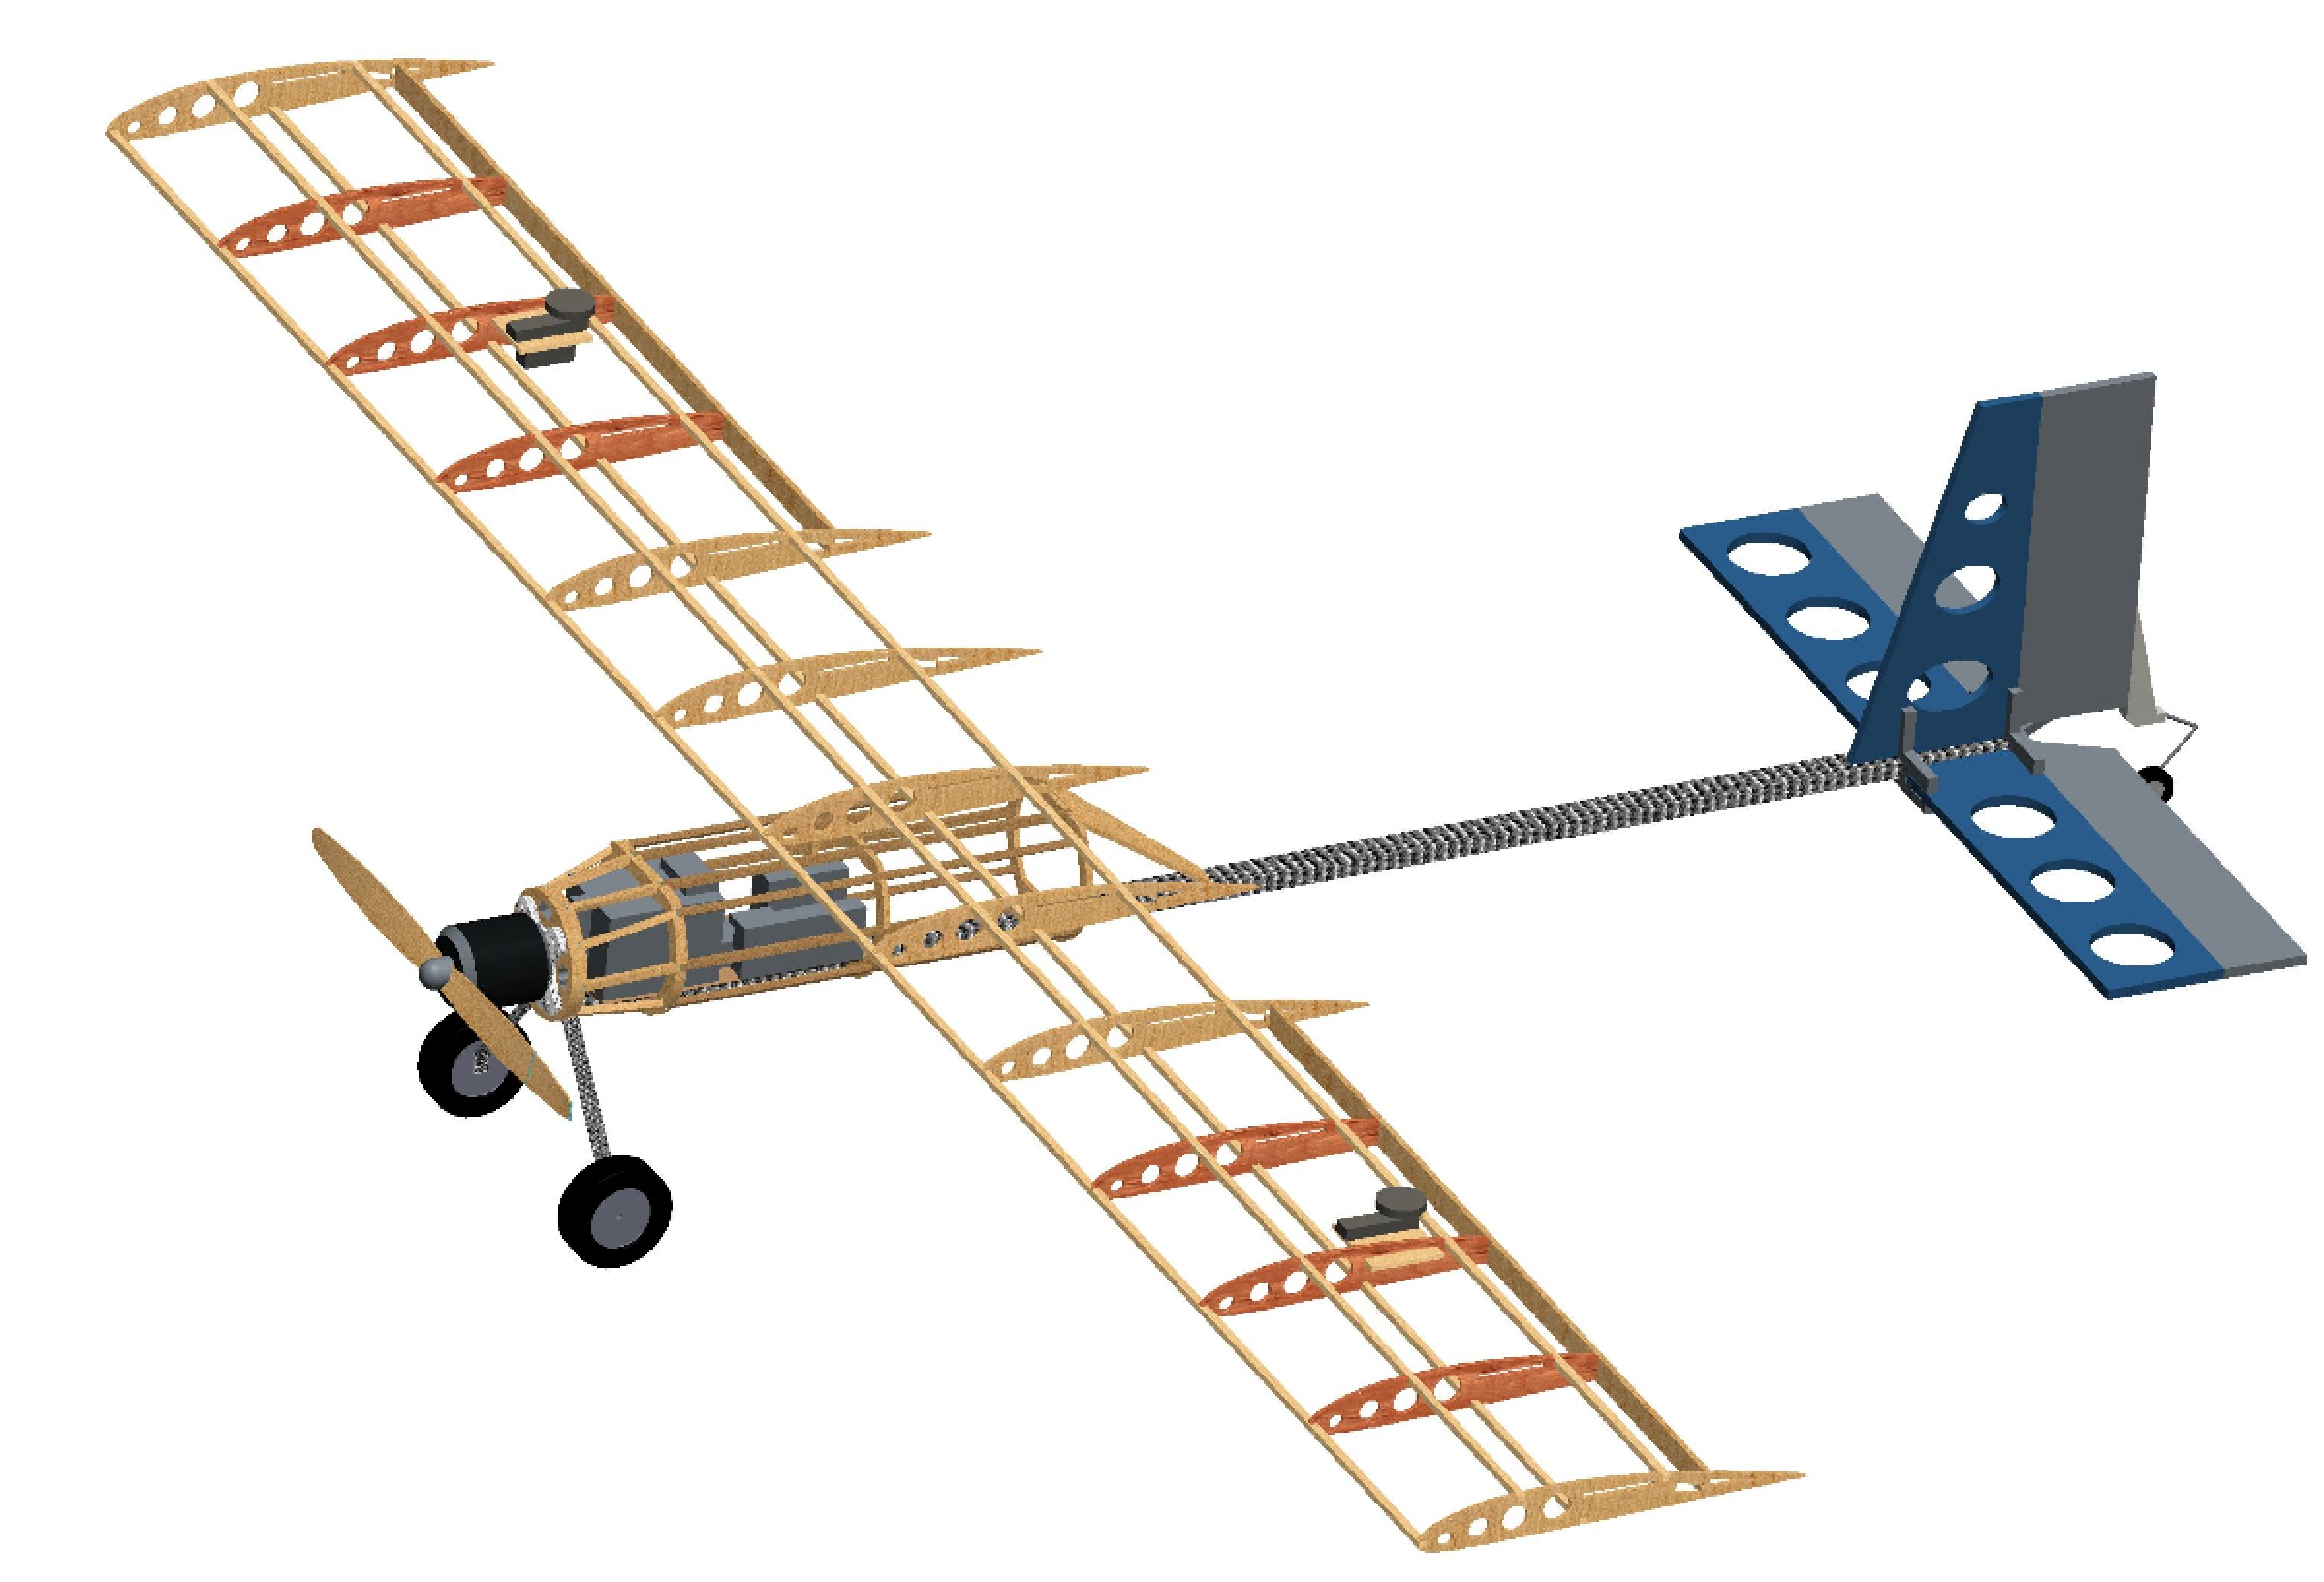
\includegraphics[width=1\columnwidth]{Full_No_Caption.jpg}
\caption{Isometric view of CAD model highlighting minimalist airframe structure}
\label{noskin}
\end{figure}
These material savings along with use of light woods such as balsa and spruce allowed the Team to construct a robust aircraft with a low structure weight, putting less stress on the motor during climb and requiring less of the wing during the descent glide.

To further address the issue of weight, a rectangular carbon fiber rod was chosen as the main structural element of the fuselage. As the backbone for both the fuselage and tail assemblies, the rod would take most of the stress on the airframe during flight, but would do so with minimal added weight. The fuselage was approximately cylindrical, tapering off in roughly a cone at the trailing edge and built up from the carbon fiber rod that ran through the length of its underbelly. It also housed most of the internal electronics with the exception of two aileron servos and a pitot tube in the main wing. Protruding from the front of the fuselage structure was a double-thick bulkhead upon which the motor and propeller assembly were affixed.

Located under the fuselage and epoxied directly to the front end of the carbon fiber rod, the main landing gear, experienced the most stress of any component on the aircraft due to its direct impact with the ground on landing attempts, and thus was attached strongest part of the aircraft allowing the gear system to transfer energy out of its legs upon impact. The connection points to the fuselage were also reinforced with a plywoord box, epoxied to the carbon fiber on both sides of the gear, to prevent any torquing motions from ripping the gear off of the aircraft. At the aft end of the aircraft, a small, steerable wheel was attached directly to the rudder, reducing the number of mechanical linkages and improving the takeoff performance due to the increase angle of attack of the wing while rolling on the ground. Attaching the wheel to the rudder negligibly reduced the ground control of the aircraft but improved weight characteristics, which was more desirable for the given mission profile.

The secondary driver employed in this design was a high lift-to-drag performance ratio. As outlined in the course textbook, a high lift force with a correspondingly low drag force promotes a lower descent rate during the gliding phase of flight, allowing the aircraft to remain aloft for proportionally longer periods of time. Although drag is a phenomena affecting all parts of the aircraft structure, the design of the main wing was of greatest concern to the Team as it has the largest overall effect on the ratio and, consequently, was the most challenging and, arguably, most important aspect of the design. 

Climb and glide are located at the opposite ends of the design spectrum when seeking an optimimum aspect ratio for a main wing. A small aspect ratio will help with climb and maneuverability while a large aspect ratio increases the performance during glide. To address each of these, an aspect ratio of 7 was selected to strike a mean between the two extremes, leading to a total wing span of 66 inches and a constant chord length of 9.6 inches. These design characteristics were implemented using a Clark Y flat-bottom airfoil. Used extensively in remote-controlled aircraft applications, the flat bottom afforeded the Team the ability to attach a mounting plate to the underside of the wing, allowing it to rigidly screw down onto the fuselage structure. The Clark Y also has the advantage of excellent lifting qualities at the low to middle range angles of attack at which the aircraft would be flying. A detailed drawing depicting the Clark Y shape and the rib structure of the aircraft can be found below in Figure \ref{wing} which also highlights the dimensions of the main wing structure.

\begin{figure}[h]
 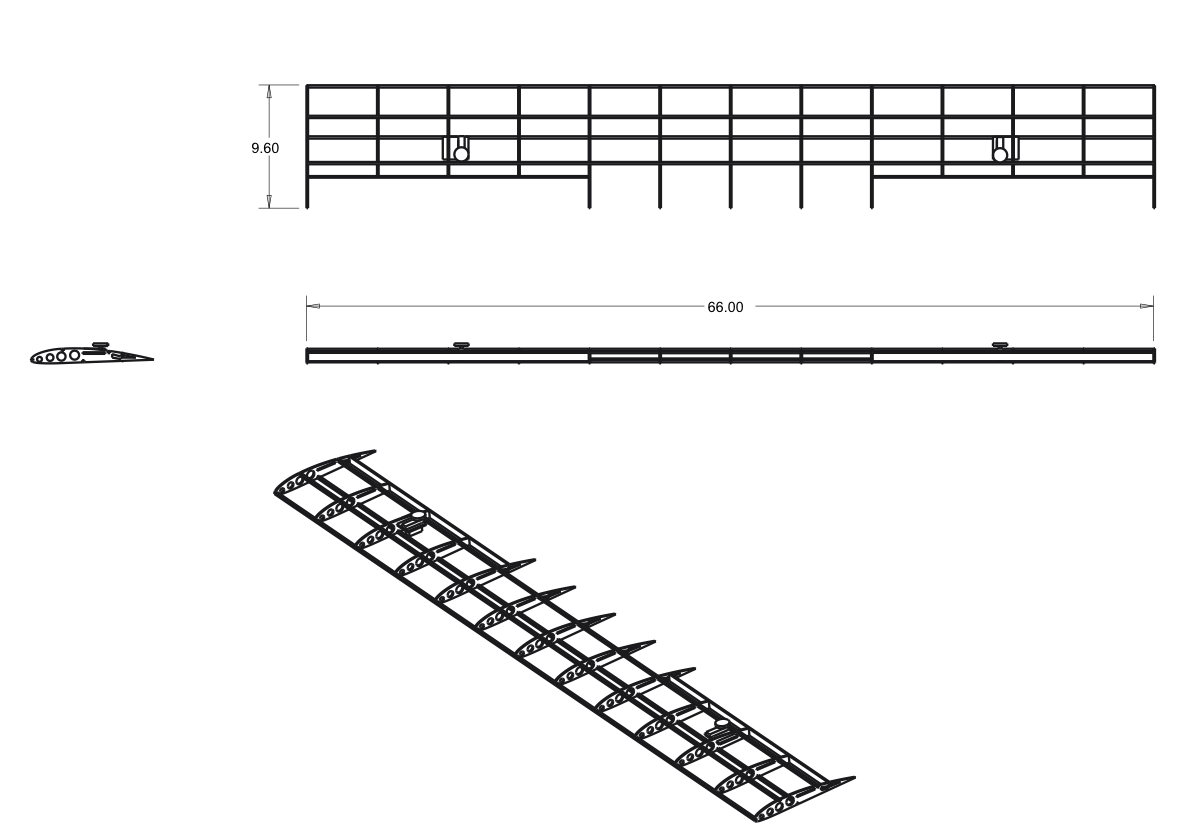
\includegraphics[width=1\columnwidth]{Wing_Design.png}
 \caption{Dimensioned model of the main wing depicting rib structure as well as airfoil shape and positioning.}
\label{wing}
\end{figure}

The tail was of conventional design placed at the free end of the carbon fiber rod protruding from the fuselage as seen in Figure \ref{noskin}. One of the main concerns of this design, however, was the potential for severe torquing from the lift forces generated by the tail surfaces. Addressing these issues early in the design process, the thickness of the carbon fiber rod was doubled, as was the thickness of the plywood used to construct the tail surfaces, leading to structurally sound design as seen in Figure \ref{tail} below, which also highlights the main dimensions, in inches, of the horizontal and vertical tail surfaces. A custom bracket was designed for the attachment of the tail surfaces to the carbon fiber, and each tail surface was anchored, using epoxy, to the bracket at two locations, thus preventing twisting. The elevator and rudder control surfaces were overdesigned to provide more than sufficient control of the aircraft and prevent flutter or twist in-flight. Although Figure \ref{tail} shows large holes in the tail surface, these were monokoted over in the final design, allowing weight savings without any detriment to performance.

\begin{figure}[h]
 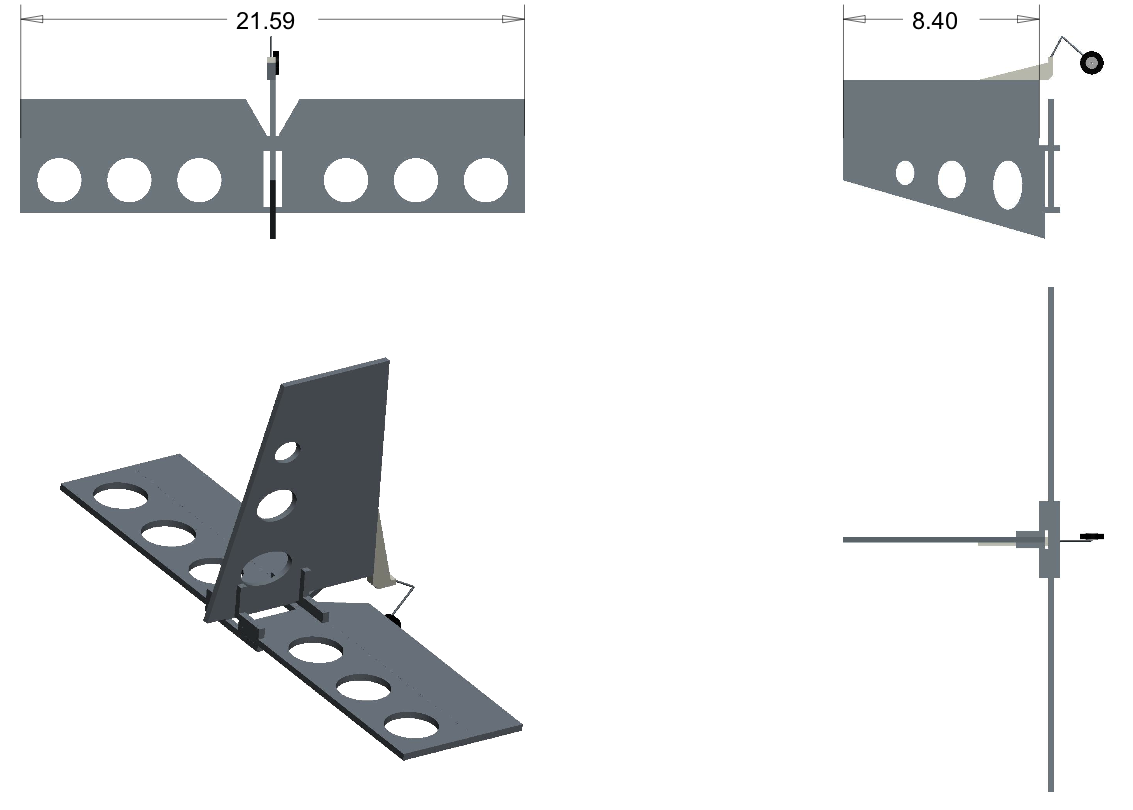
\includegraphics[width=1\columnwidth]{Tail_Design.png}
 \caption{Tail design detailing important dimensions and weight-saving structural designs.}
\label{tail}
\end{figure}
 
Rouding out the design, the aircraft used a 1.25 horsepower motor, capable of providing approximately 3.5 pounds-force of thrust. With a final takeoff weight of 5 pounds, including a 0.84 pound payload, this yielded a final thrust-to-weight ratio of 0.7. The motor powered a 13-inch propeller with an 8-inch pitch which created the power to move the craft through the air. As the main wing was bolted onto the fuselage before flight, hatches in both the top and side of the fuselage were used to allow access to internal components without removing the wing. The final flight vehicle is shown below in Figure \ref{real} in a picture taken just seconds after the final component of the fuselage was added, completing the craft.

Design characteristics of the aircraft were chosen using a Figure of Merit analysis, detailed and tabularized in Appendix A. The Figure of Merit analysis assigns numerical weights to different component designs based on drivers such as weight and size. The component with the most favorable weighting and ease of construction was the one chosen for use in the design.
\begin{figure}[h]
 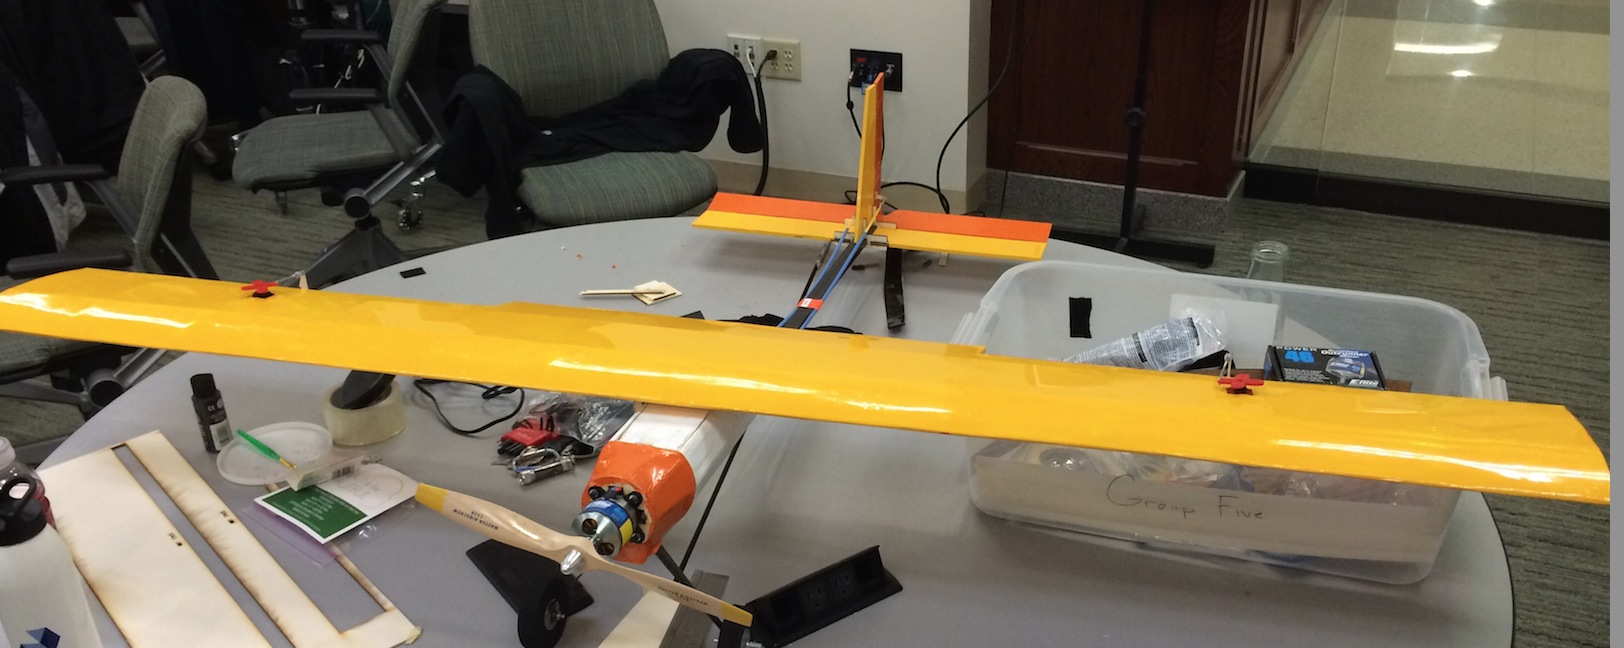
\includegraphics[width=1\columnwidth]{Real_Wing.jpg}
 \caption{Flappy Bird aircraft seconds after completion}
\label{real}
\end{figure}

\section{Predictions from Spreadsheet Analysis}
As part of the detailed design, a series of spreadsheets were used to determine relative values for vehicle handling qualities and component design. Perhaps one of the most integral factors for determining the aircraft's ability to perform well within the mission constraints is the wing loading as it plays a significant role in both an aircraft's climb and glide performance. As mentioned previously, glide performance is the mission phase in most need of optimization and, as such, the wing loading on the vehicle was determined based on performance during descent, for which a low wing loading is desired. Assuming a ground elevation of 823 feet in Bremen, Indiana, the town in which the field is located, the wing loading during glide was predicted to amount to approximately 13 oz/ft$^2$, a value corroborated by the pilots who would be controlling the aircraft during flight testing.

Given these flight characteristics and data culled from previous years' planes, the final climb rate of the aircraft was predicted to be 1,100 feet per minute, although the Team determined early on that the actual rate would decrease due to the structure weight of the high aspect ratio wing. Over the stated ten second time interval, this climb rate predicted a gain in altitude of approximately 200 feet. Assuming the unpowered glide would begin at this altitude, it was estimated that the aircraft would lose 152 feet of altitude every minute, thus requiring approximately 78 seconds to return to its original cruising altitude. As before, this glide rate assumes ideal flight conditions and is expected to diminish somewhat during flight testing. While at level flight, the design parameters in the spreadsheet predicted a cruising speed of 44 miles per hour.

Those spreadsheets that were used in the design process are attached at the back of this report as Appendix B. It should be noted that these were used merely as guides for ranges of acceptable values and, in many cases, actual design decisions were made based on input from both the pilots and teaching assistants who pulled design advice from previous experience.

\section{Flight Test Results}
During flight testing, the Flappy Bird flew a total of two test runs, each following the three phases of the mission profile. To numerically track the performance of the aircraft on these flights, altitude and speed data were collected by an onboard sensor package, including a pitot static tube mounted starboard wing tip. After eliminating the data collected while the plane was readied for flight, Figure \ref{Trial}, containing altitude data over each test flight, and Figure \ref{speed}, a graphic showing the speed of the aircraft during its flight testing, were produced to give a reader a visual representation of the information collected during flight testing.

\begin{figure}[h]
 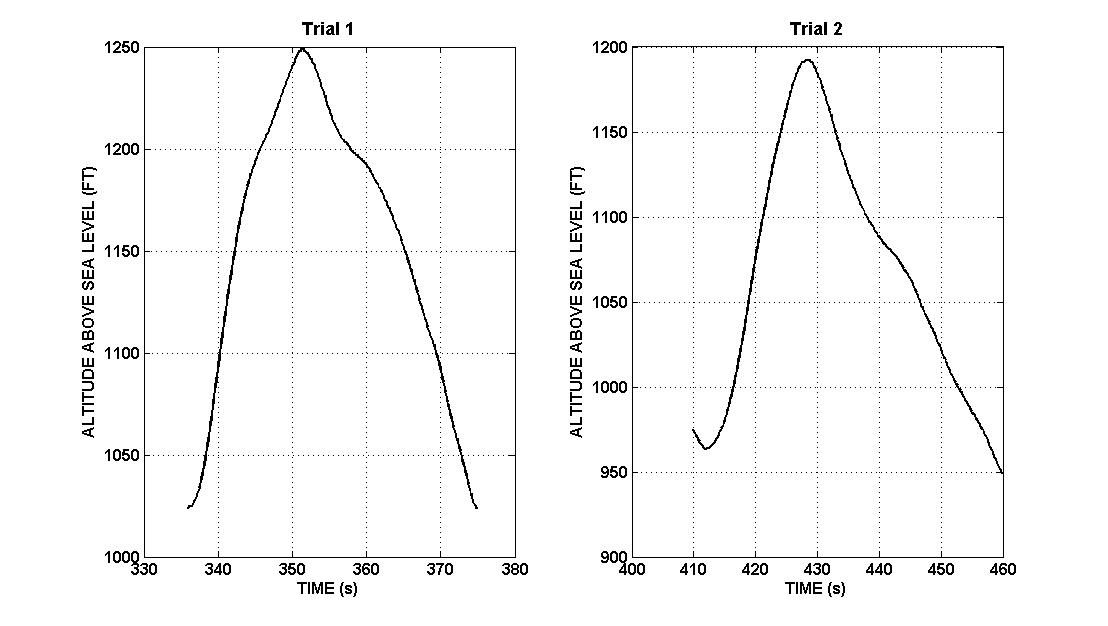
\includegraphics[width=1\columnwidth]{FlightTrialPlots.jpg}
 \caption{Climb and descent profiles flown by the Flappy Bird aircraft during two flight tests.}
\label{Trial}
\end{figure}

\begin{figure}[h]
 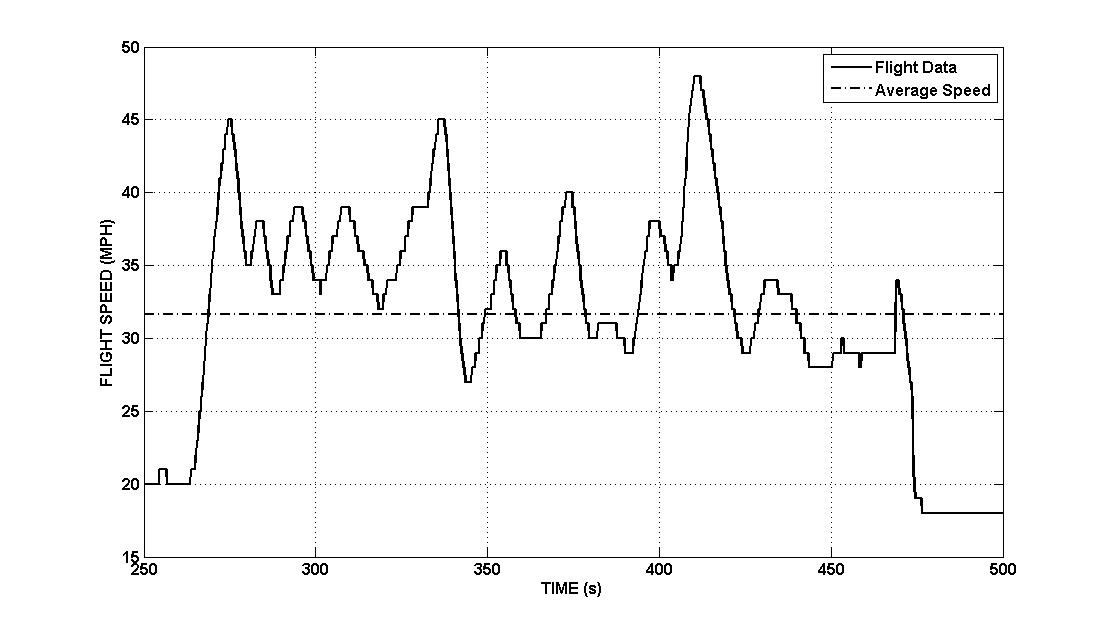
\includegraphics[width=1\columnwidth]{speed.jpg}
 \caption{Speed of Flappy Bird aircraft measured by onboard sensors throughout flight test.}
\label{speed}
\end{figure}

Focusing first on Figure \ref{Trial}, one can easily see that the climb and glide performance were similar through both test flights. In Trial 1, the aircraft was able to make a rapid ascent to an altitude of 1250 feet above sea level, or approximately 400 feet above the ground before gliding back to its original cruising altitude in a time interval of 24 seconds. In Trial 2, the pilots were able to make a more uniform climb up to the aircraft's peak altitude of 1900 feet above sea level before gliding back down to altitude in 26 seconds. 

Using this data, the Team was able to calculate rates for both ascent and descent for the two flight profiles. The maximum rate of climb for this aircraft, 1246 ft/min occured in the first leg of the ascent in Trial 1 as illustrated by the steep gradient from the cruising altitude to approximately 1200 ft. That ascent also saw the lowest rate of climb, 548 ft/min, during the final climb from 1200 feet to 1250 feet in altitude.

In a similar manner, the Team also conducted an analysis of descent, or glide, rates. As depicted clearly in the Trial 2 diagram of Figure \ref{Trial}, the final leg of descent, from approximately 1050 ft to the cruising altitude, represents the slowest measured rate of descent of the aircraft at 405 ft/minute. This was counteracted by a 596 ft/min descent rate between 1200 ft and the cruising altitude in Trial 1.

Each of the two trials depicted in Figure \ref{Trial} took place during a single, continuous test flight. Therefore, Figure \ref{speed}, upon which focus will now be placed, depicts the aircraft speed through both trials from first takeoff to final landing. As the horizontal dashed line indicates, the mean speed of the aircraft during its test flights was 31.6 mph, a number clearly affected by the low-speed regions of the figure surrounding takeoff and landing. During the flight, however, the aircraft also reached a peak speed of 48 mph, showing that speeds like the 44 mph predicted by the spreadsheet were, in fact, possible with this aircraft.  

Using this flight data the figure of merit for the flight testing, the success factor, was calculated using the formula presented in Equation \ref{success} as

\begin{equation}
S = (dH/dt)_c + (dH/dt)_g - \Delta(dH/dt)_c - \Delta(dH/dt)_g,
\label{success}
\end{equation} 
where $(dH/dt)$ represents the rate of climb or glide, identified by the subscripts ``c" and ``g", respectively, and $\Delta(dH/dt)$ represents the absolute difference between the predicted and actual rates of climb and glide following the same subscript identifications as before. After calculating each of these quantities, the flight success factor was determined to be 441.94 ft/min, approximately 47 \% of the success factor of 947.66 ft/min calculated assuming a perfect ascent and descent using the numbers produced by the design spreadsheets.

\section{Discussion}
For a first iteration of a design idea, the Flappy Bird performed admirably during its flight testing and proved an airworthy and highly maneuverable aircraft. As the success factor indicates, however, further iterations would require that work be done to improve its performance in a few key areas. As mentioned in Section \ref{design}, the two primary design drivers were geared towards optimizing the glide rate of the aircraft, an area in which the aircraft, admittedly, struggled. Its performance in this area, however, is well explained.

On the day of flight testing, strong winds were predicted and observed at the field during most of the flight test runs, this test proving no exception. Although these winds were within the acceptable limits of flying, they did have a deleterious effect on the rates of climb and glide due to their negative effects on the lifting surfaces. During ascent to the peak altitude, the pilots chose to climb at an angle of attack lower than might have normally been pursued to prevent the wind from causing a nose up moment that might stall the wing. Therefore, the rates shown in Figure \ref{Trial} may not necessarily be representative of the full capabilities of the aircraft. Similarly for glide, although the pilots attempted to fly into the wind to gain favorable lift performance, strong updrafts continued to push the wing towards stall, necessitating that they enter onto a steeper glide slope than might otherwise have been possible. The pilots, however, push the plane to the best acceptable limits during their flight so the data presented, although possibly skewed by the wind, represents the aircraft's best performance in adverse conditions.

The weather is not the sole focus of analysis for the aircraft as improvements could also be made in the design itself. If one recalls, aircraft weight was the primary design driver for the Flappy Bird aircraft, a decision that ultimately led to the minimalist design flown on the flight day. During the conceptualization process, this arrangement was predicted to fare well in both climb and glide, allowing the Team to strike a balance between climb and glide performance. If one recalls the mission profile, a fast climb, gained by a high thrust-to-weight ratio, would permit the Flappy Bird to reach a substantial altitude at the end of 10 seconds, permitting a longer glide time by increase the distance through which the aircraft would have to glide to level off back at its cruising altitude. The weight, coupled with the high aspect ratio, low wing loading main wing would also help to improve the glide performance by increasing the lift on the main wing through the entirety of the gliding phase. When physically constructed, however, the small fuselage and its limited exterior surface area, created a design challenge for the Team to place the main wing and components such that the aircraft remained stable during flight and maintained an acceptable margin between the center of lift on the main wing and the center of gravity of the aircraft as a whole. Through creative use of the wall and floor surfaces, this margin was obtained, but it provided only a small travel between stable and unstable, possibly creating more issues for the pilots during flight.

Despite the design and performance issues, most of which were anticipated, the aircraft did manage to yield a large success factor. As Equation \ref{success} indicates, the success factor is determined by both climb and glide rates. Previous senior design aircraft appeared to all perform climbs at rates approaching 1100 ft/min and, given the Team's design for the Flappy Bird, rates in the top end of the historical data were thought to correspond better with the performance characteristics that the aircraft catered to. As the flight test data indicates, not only was the aircraft capable of reaching that 1100 ft/min speed, but was actually able to climb at a rate significantly faster than that predicted even despite the strong winds. Although this climb rate was not maintained throughout the ten second interval, it allowed the aircraft to reach an altitude of 1250 ft above sea level, placing it in an advantageous position to begin its glide. As mentioned previously, there were many factors that contributed to a lower average climb rate throughout the two test flights, but the Team believes it can deem the flight a success because the aircraft surpassed the original predictions which were made assuming perfect flight conditions.

Although the success in glide was not as pronounced as that in climb, the Team still believes that the results are not as unexpected as one might first believe. The spreadsheet analysis, again, conducted assuming perfect, calm flight conditions, placed the Flappy Bird's minimum descent rate at 152 feet of altitude lost for every minute of flight, a value which was over three times less than the minimum descent rate of 405 ft/min observed on flight day. The team did not, however, expect to reach this low glide value simply because of the imperfection of the design. When assuming a perfect wing section in the spreadsheets, wind is assumed to flow over the airfoil surface without any perturbations or abberations, leaving a smooth boundary layer and a consistent lift on the airfoil. Although the smooth surface was achieved using monokote over the wing, possible imperfections in the both the airfoil design and its attachment scheme to the fuselage assuredly led to a fractional loss in lift not able to be reproduced on spreadsheets which did not take into account any of the finer design details of the aircraft, leading to the lower-than-predicted results. Regardless of this fact, the Team stresses that, for a basic first design, the flight testing went extremely well, leaving the aircraft with 47 \% of its intended success design and only falling short in areas for which the imperfections are well-explained and well understood. 

\section{Conclusion}
When any new vehicle of component design begins to take shape at any aerospace company, every detail is meticulously analyzed using both computational and physical test methods to ensure the final product is safe for customers and reliable for its stated design mission. Although scale model aircraft, such as those used in this project, do not fall under such stringent requirements, the need to verify design is key in both situations. The Flappy Bird aircraft was very much a conceptual design turned physical model flown for the purposes of demonstrating basic knowledge of flight principles and aerodynamic theory and, by all accounts, the aircraft succeeded in its purpose. Not only was the vehicle able to successfully takeoff and land under its own power, but during flight was proven to be highly maneuverable and exceeded expections in climb performance. For a first design iteration, however, the losses observed in glide were acceptable and easily addressed in subsequent design were there to be more. 

The benefit of remote-controlled aircraft is the minimal price paid for possible performance issues. Whereas commercial aircraft components may cost thousands of dollars to test and validate, the kits used in this project cost a minuscule fraction of that, promoting daring designs and welcoming issues as an opportunity to learn. Therefore, although the flight data was not always as predicted, it provided the impetus to return to the conceptual design of the aircraft to identify areas in which the physical structure and performance characteristics of the aircraft could be improved if the vehicle were to be redesigned. The most important takeaway, however, is that the aerospace education gained thus far has allowed the Team to construct a vehicle capable of flight and capable of meeting a specific mission profile with tools taught in the classroom, providing motivation to seek out design opportunities in the commerical industry but also providing confidence to the engineers that their education is applicable to real-world design problems and their experience is broad enough to enable them to address and solve problems that may occur throughout the process.

\newpage

\begin{appendices}
\section{Figure of Merit Analysis}
Although this design is ultimately constrained by the requirements of the mission statement, a determination of favorable attributes for an aircraft of this type was conducted using a figure of merit (FoM) analysis. An FoM analysis is part of a design approach that is used to select components that form an aircraft's structure in an efficient and objective manner. Although the analysis cannot produce design dimensions, it can provide a numerical point of comparison between different variations of airframe components under consideration. As Table \ref{tab:FoMGen} shows, physical and performance characteristics are evaluated across a rating system between 1 and 5, with larger numbers representing a greater importance to the design drivers. The row totals are then summed and each characteristic is assigned a bias percentage which determines its overall priority in the final design. 


\begin{table}[h!]
\caption{Figures of Merit for Aircraft Performance}
\resizebox{\textwidth}{!}{%
\begin{tabular}{|c|c|c|c|c|c|c|c|c|}
\hline
 & \textbf{Weight} & \textbf{High L/D} & \textbf{Size} & \textbf{Ease of Construction} & \textbf{Stability \& Control} & \textbf{Payload} & \textbf{Row Totals} & \textbf{Bias} \\
\hline
\textbf{Weight} & 0.00 & 4.00 & 4.00 & 4.00 & 4.00 & 5.00 & 21.00 & 23 \% \\
\hline
\textbf{High L/D} & 2.00 & 0.00 & 4.00 & 4.00 & 3.00 & 5.00 & 18.00 & 20 \% \\
\hline
\textbf{Size} & 2.00 & 2.00 & 0.00 & 2.00 & 2.00 & 2.00 & 10.00 & 11 \% \\
\hline
\textbf{Ease of Construction} & 2.00 & 2.00 & 4.00 & 0.00 & 1.00 & 3.00 & 12.00 & 13 \% \\
\hline
\textbf{Stability \& Control} & 3.00 & 3.00 & 4.00 & 5.00 & 0.00 & 4.00 & 19.00 & 21 \% \\
\hline
\textbf{Payload} & 1.00 & 1.00 & 4.00 & 3.00 & 2.00 & 0.00 & 11.00 & 12 \% \\
\hline
\end{tabular}}
\label{tab:FoMGen}
\end{table}

Once the design biases have been set, the figure of merit analysis is conducted on each of the possible component configurations considered for the final design. Table \ref{tab:wing} illustrates the process for the main wing selection. Unlike Table \ref{tab:FoMGen}, component analyses ratings are based on each configuration's benefit or detriment to the stated design drivers, with larger numbers representing more beneficial performance. These rankings are based on research into each possible configuration with special care taken to identify the strengths and weaknesses of each design. To finally determine the most appropriate component variation for the mission profile, a weighted average of the figures of merit for each configuration was tabulated, appearing on the bottom row of the matrix. Matrices for each of the other component analyses are located in Tables \ref{tab:control}-\ref{tab:motor}.

\begin{table}[h!]
\caption{Wing Design Matrix}
\resizebox{\textwidth}{!}{%
\begin{tabular}{|c|c|c|c|c|c|c|}
\hline
& \textbf{Monoplane} & \textbf{Biplane} & \textbf{Tandem Wing/Canard} & \textbf{Flying Wing/Blended Body} & \textbf{Winglets} & \textbf{Bias} \\
\hline
\textbf{Weight} & 4.00 & 3.00 & 3.00 & 5.00 & 5.00 & 23 \% \\
\hline
\textbf{High L/D} & 3.00 & 4.00 & 3.00 & 3.50 & 2.00 & 20 \% \\
\hline
\textbf{Size} & 3.00 & 1.00 & 3.00 & 4.00 & 5.00 & 11 \% \\
\hline
\textbf{Ease of Construction} & 5.00 & 2.00 & 2.00 & 1.00 & 5.00 & 13 \% \\
\hline
\textbf{Stability \& Control} & 4.50 & 3.00 & 2.00 & 1.00 & 1.00 & 21 \% \\
\hline
\textbf{Payload} & 3.00 & 3.00 & 3.00 & 1.50 & 3.00 & 12 \% \\
\hline
\textbf{Column Average} & \textbf{\underline{3.81}} & \textbf{2.85} & \textbf{2.66} & \textbf{2.81} & \textbf{3.33} & \\
\hline
\end{tabular}}
\label{tab:wing}
\end{table}

The results of each analysis were not entirely unexpected given the common history of these types of aircraft. Table \ref{tab:wing} shows that the single wing is the most advantageous wing configuration because of its low weight and relative ease of construction. Beyond those, it also boasts a high level of stability and average scores in all of the remaining categories, highlighting it as the best possible configuration.

Scoring highly in the same categories as the wing, the conventional tail also logged a markedly higher score than its competitors. Historical data comparisons show that the conventional tail has the lowest weight of the three variations in the category and, due to its right angle mounted design, scores well for ease of construction as well.

The final component selection of note is that of the landing gear. Historically, the three wheel trike configuration has a heavier under-mount system than other options such as the skids and tail gear which would suggest that it would conflict with the primary design driver of weight. In this instance, however, the additional stability gained over other gear options provided enough justification to the team to prioritize stability over weight. In addition to stability advantages, the trike gear also provides the aircraft with a more forgiving structure on which to land and takeoff. The three wheel configuration elevates the underbelly off the ground and provides some level of shock absorption during landing, preventing damage to the fuselage or lifting surfaces. 

\begin{table} [h!]
\caption{Control Surface Component Matrix}
\resizebox{\textwidth}{!}{%
\begin{tabular}{|c|c|c|c|c|c|}
\hline
& \textbf{2 Ailerons, 2 Elevators, 2 Flaps} & \textbf{2 Ailerons, 1 Elevator, 2 Flaps} & \textbf{2 Ailerons, 2 Elevators} & \textbf{Two Elevons} & \textbf{Bias} \\
\hline
\textbf{Weight} & 1.00 & 2.00 & 3.00 & 5.00 & 23 \%\\
\hline
\textbf{High L/D} & 5.00 & 4.00 & 3.00 & 1.00 & 20 \% \\
\hline
\textbf{Size} & 1.00 & 2.00 & 3.00 & 5.00 & 11 \% \\
\hline
\textbf{Ease of Construction} & 1.00 & 1.00 & 3.00 & 5.00 & 13 \% \\
\hline
\textbf{Stability \& Control} & 2.00 & 2.00 & 4.00 & 1.00 & 21 \% \\
\hline
\textbf{Payload} & 0.00 & 0.00 & 0.00 & 0.00 & 12 \% \\
\hline
\textbf{Column Average} & \textbf{1.88} & \textbf{2.02} & \textbf{\underline{2.85}} & \textbf{2.77} & \\
\hline
\end{tabular}}
\label{tab:control}
\end{table}


\begin{table}[h!]
\caption{Landing Gear Component Matrix}
\resizebox{\textwidth}{!}{%
\begin{tabular}{|c|c|c|c|c|c|c|c|}
\hline
& \textbf{None} & \textbf{Trike} & \textbf{Skids} & \textbf{Retractable} & \textbf{Tail} & \textbf{Monowheel} & \textbf{Bias} \\
\hline
\textbf{Weight} & 5.00 & 3.00 & 4.00 & 1.00 & 3.50 & 4.00 & 23 \%\\
\hline
\textbf{High L/D} & 5.00 & 3.00 & 4.00 & 1.00 & 4.00 & 4.00 & 20 \%\\
\hline
\textbf{Size} & 5.00 & 3.00 & 3.00 & 1.00 & 3.50 & 4.00 & 11 \% \\
\hline
\textbf{Ease of Construction} & 3.00 & 5.00 & 3.00 & 1.00 & 4.00 & 2.00 & 13 \% \\
\hline
\textbf{Stability \& Control} & 0.00 & 5.00 & 1.00 & 3.00 & 2.00 & 1.00 & 21 \% \\
\hline
\textbf{Payload} & 0.00 & 0.00 & 0.00 & 0.00 & 0.00 & 0.00 & 12 \% \\
\hline
\textbf{Column Average} & \textbf{3.09} & \textbf{\underline{3.32}} & \textbf{2.65} & \textbf{1.30} & \textbf{2.93} & \textbf{2.63} & \\
\hline
\end{tabular}}
\label{tab:gear}
\end{table}

\newpage 

\begin{table}[h!]
\caption{Tail Configuration Matrix}
\centering
\begin{tabular}{|c|c|c|c|c|}
\hline
& \textbf{Conventional} & \textbf{V-Tail} & \textbf{H-Tail} & \textbf{Bias}\\
\hline
\textbf{Weight} & 4.00 & 4.00 & 2.00 & 23 \%\\
\hline
\textbf{High L/D} & 5.00 & 5.00 & 2.00 & 20\%\\
\hline
\textbf{Size} & 3.00 & 3.00 & 2.00 & 11 \% \\
\hline
\textbf{Ease of Construction} & 5.00 & 2.00 & 5.00 & 13 \% \\
\hline
\textbf{Stability \& Control} & 4.00 & 2.00 & 5.00 & 21 \% \\
\hline
\textbf{Payload} & 3.00 & 3.00 & 3.00 & 12 \% \\
\hline
\textbf{Column Average} & \textbf{\underline{4.10}} & \textbf{3.29} & \textbf{3.14} & \\
\hline
\end{tabular}
\label{tab:tail}
\end{table}

\begin{table}[h!]
\caption{Motor Configuration Matrix}
\centering
\begin{tabular}{|c|c|c|c|}
\hline
& \textbf{Mono-Tractor} & \textbf{Mono-Pusher} & \textbf{Bias}\\
\hline
\textbf{Weight} & 4.00 & 4.00 & 23 \%\\
\hline
\textbf{High L/D} & 4.00 & 2.00 & 20 \%\\
\hline
\textbf{Size} & 3.00 & 3.00 & 11 \% \\
\hline
\textbf{Ease of Construction} & 5.00 & 3.00 & 13 \% \\
\hline
\textbf{Stability \& Control} & 4.00 & 2.00 & 21 \% \\
\hline
\textbf{Payload} & 3.00 & 3.00 & 12 \% \\
\hline
\textbf{Column Average} & \textbf{\underline{3.90}} & \textbf{2.82}& \\
\hline
\end{tabular}
\label{tab:motor}
\end{table}
\newpage

\section{Design Guidance Spreadsheets}
\begin{minipage}{\textwidth}
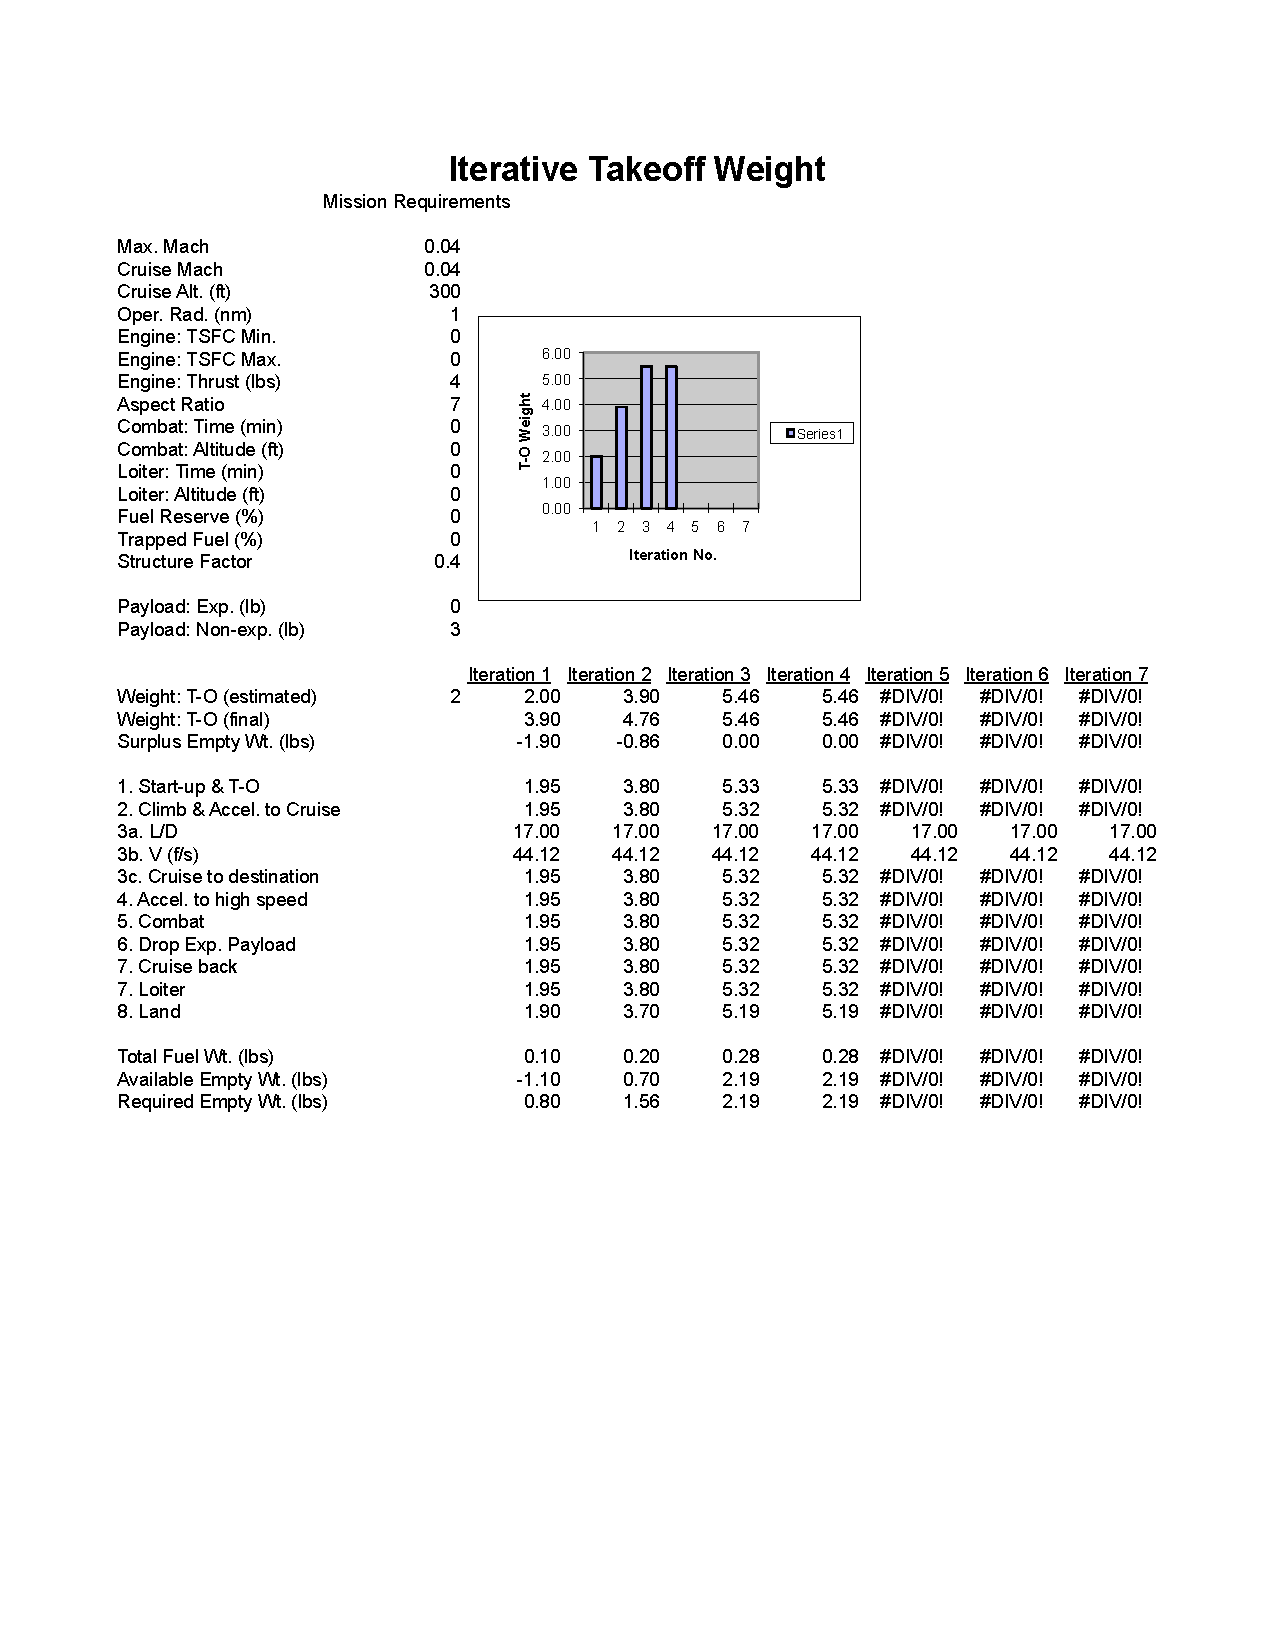
\includepdf[scale=0.9]{SpreadsheetsIterTow.pdf}
\end{minipage}
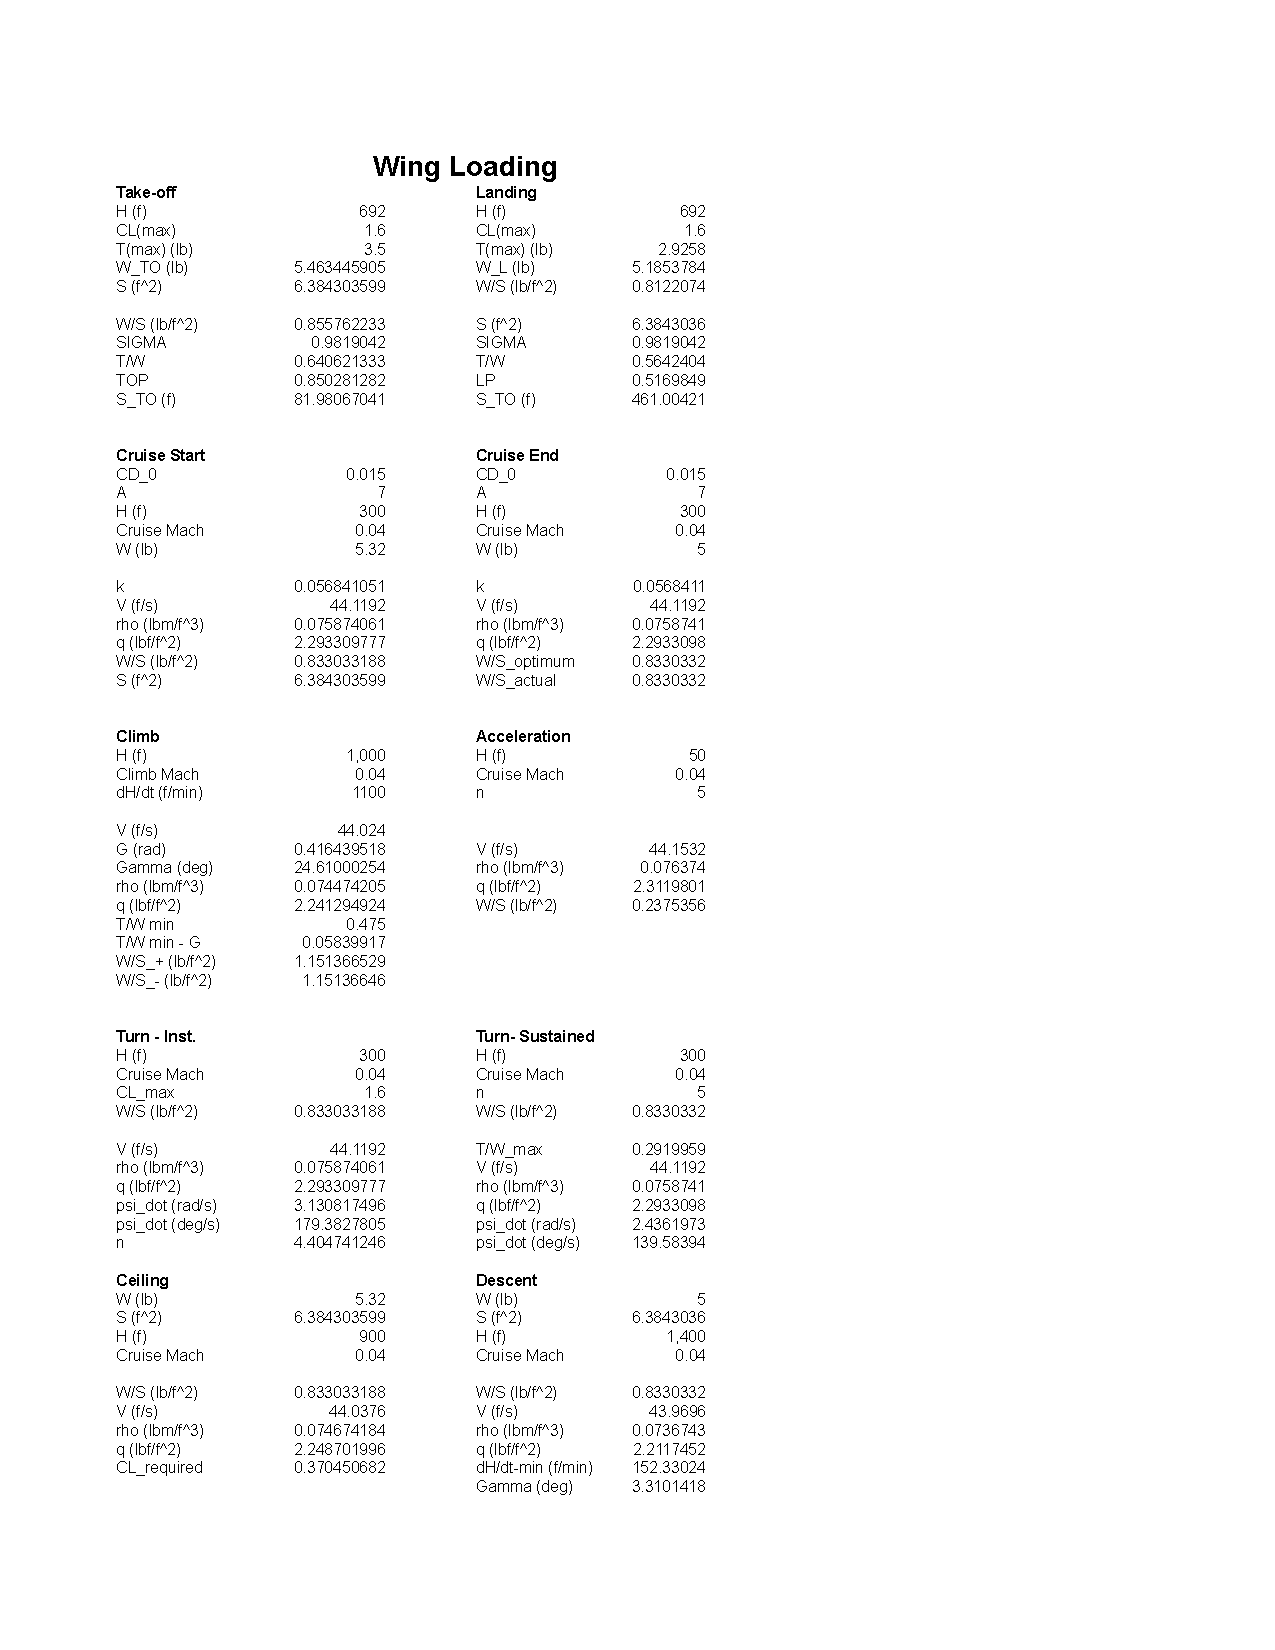
\includepdf[pages={1}]{SpreadsheetsWingLD.pdf}
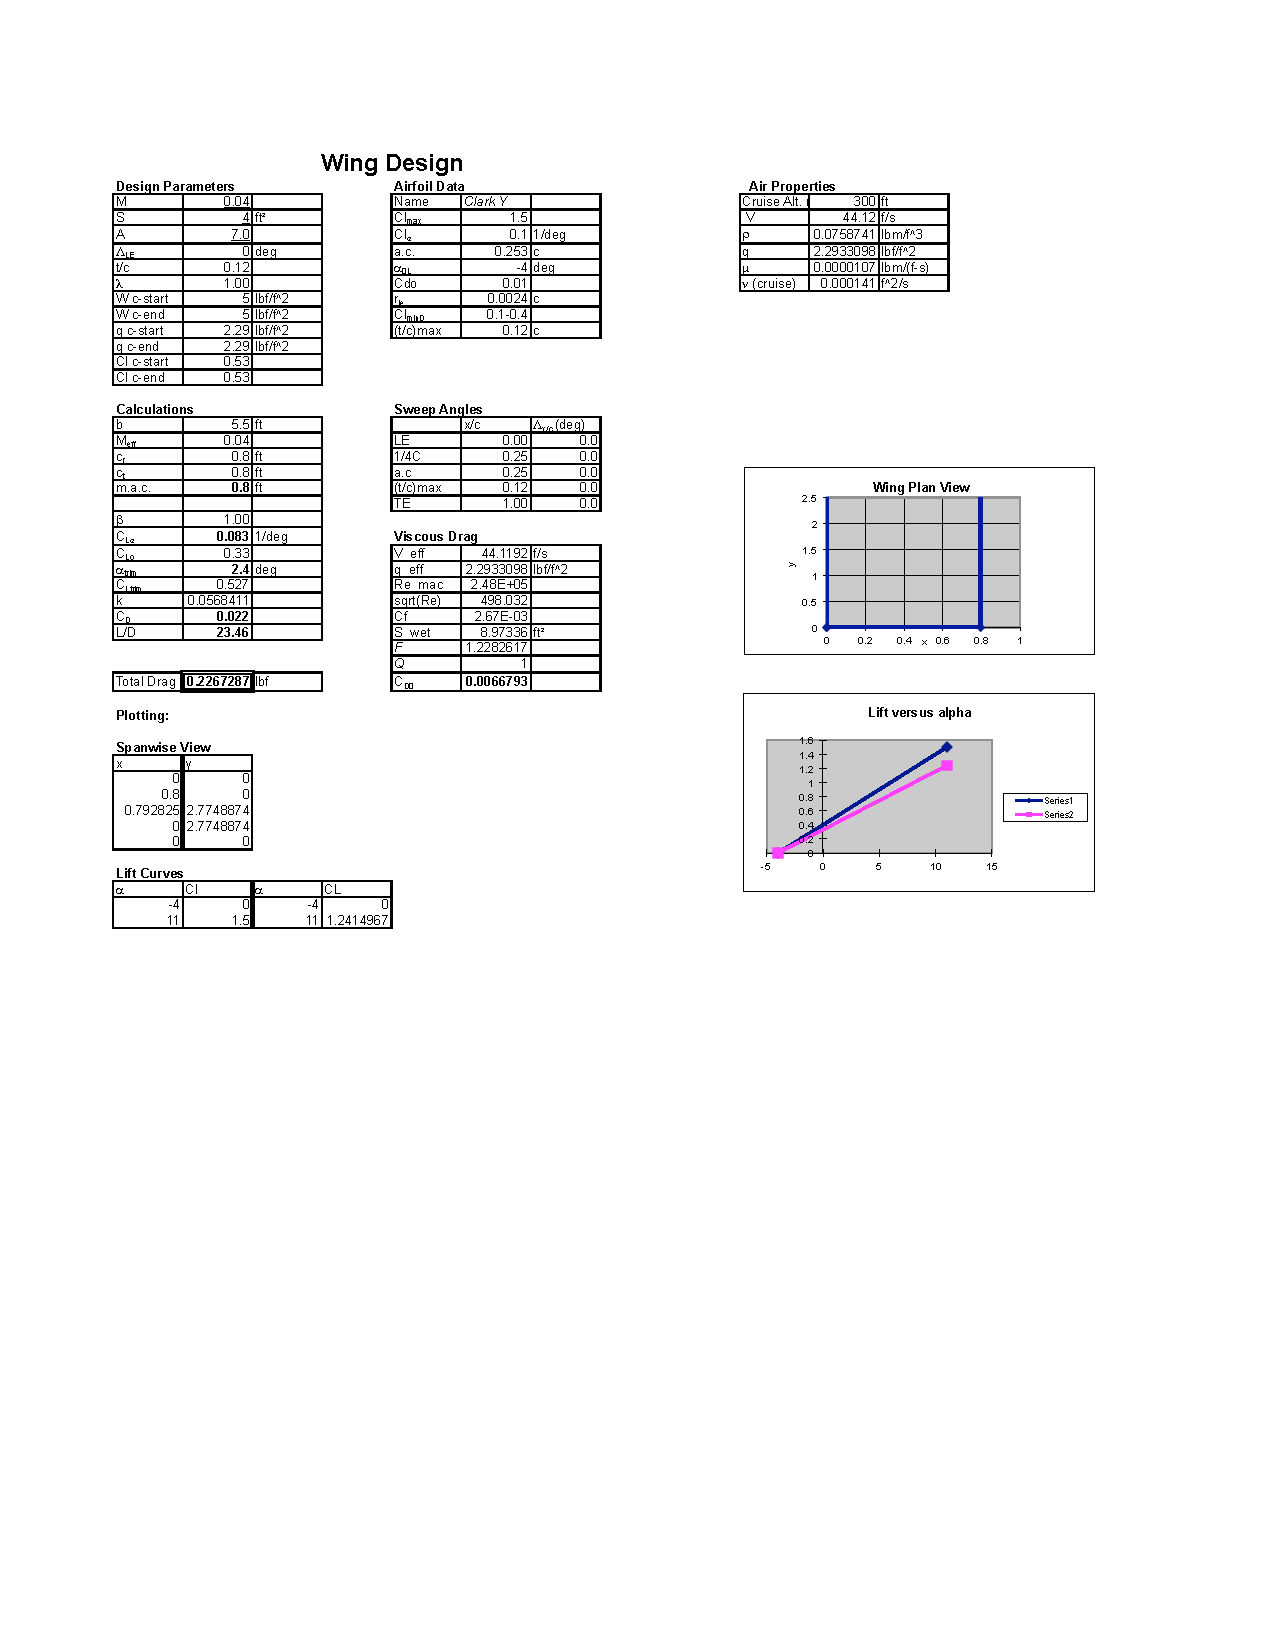
\includepdf[pages={1}]{SpreadsheetsWing.pdf}
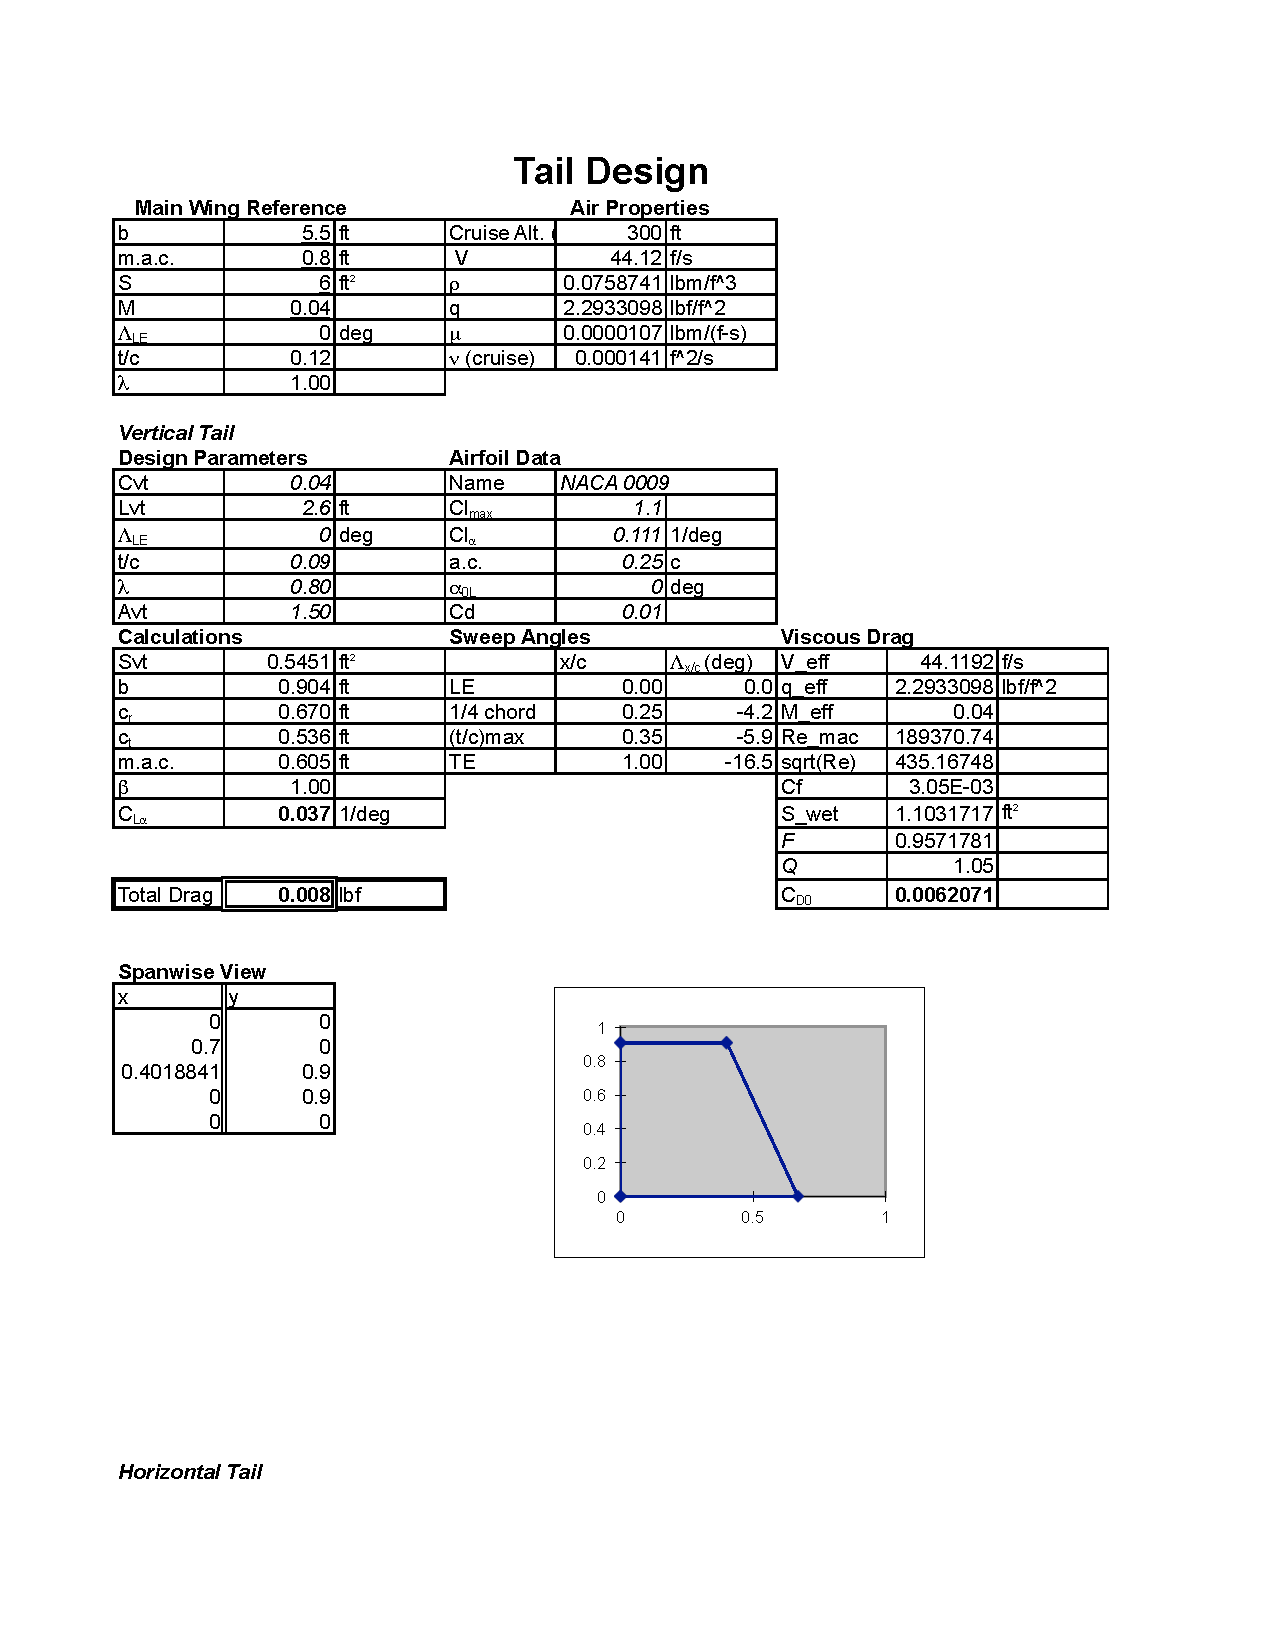
\includepdf[pages={-}]{SpreadsheetsTail.pdf}
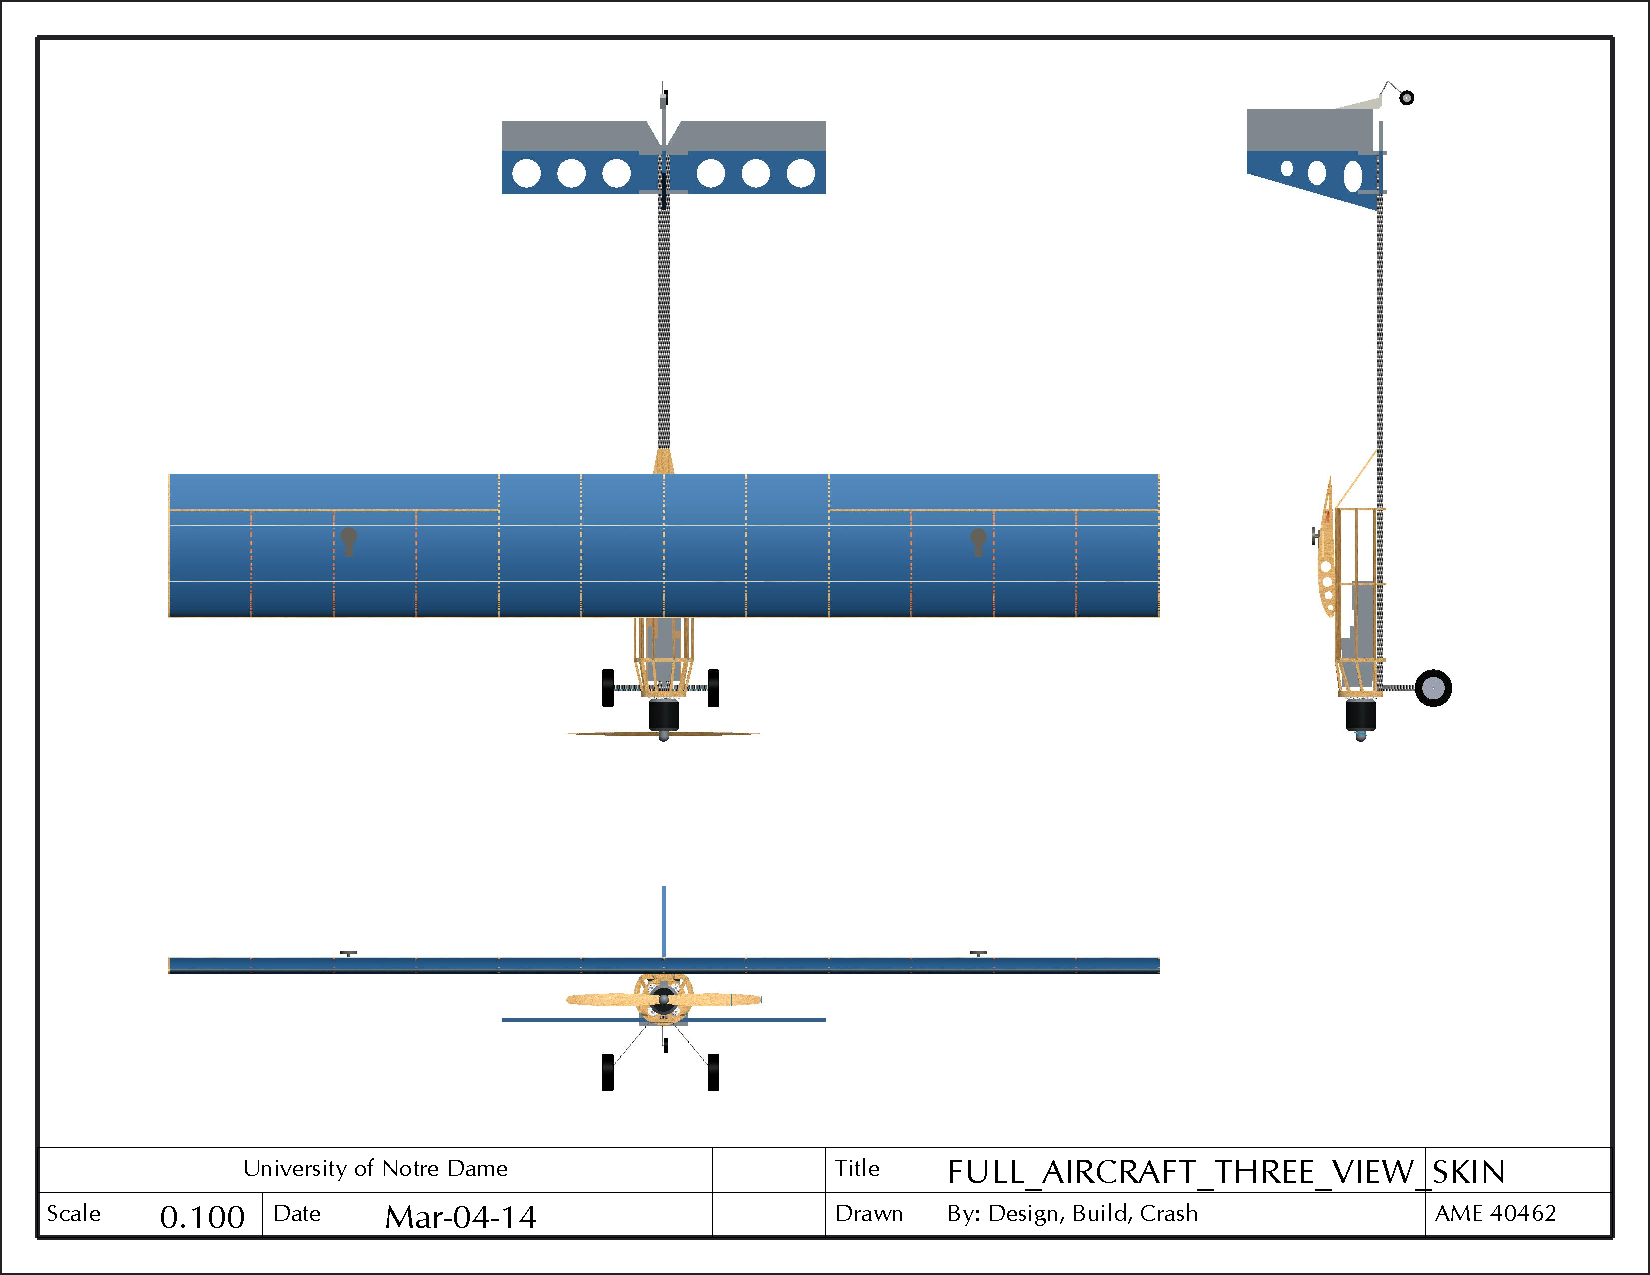
\includepdf[pages={1}]{Skin.pdf}
\end{appendices}
\end{document}